\documentclass[a4paper,oneside,UTF8, winfonts]{ctexart}
\setCJKmainfont{微软雅黑}
\usepackage{anysize} % for margin

\usepackage{fancyhdr} % for header and footer

\usepackage{ulem} %for underline

\usepackage{multirow}
\usepackage{fontawesome}

\usepackage{enumitem}
% set margin \marginsize{left}{right}{top}{bottom} 
\marginsize{2.2cm}{2.2cm}{1.3cm}{1.5cm}
% set page header
\headheight 45 true pt
\headsep 5 true pt
\footskip 25 true pt 
% set header and footer
\pagestyle{fancy}
\lhead{
\includegraphics[width=6cm,height=1.5cm]{buptlogo.jpg}}
\chead{}
\rhead{}
\lfoot{}
\cfoot{\zihao{-5} \heiti 非常感谢您百忙中的关注,真诚希望得到与您面谈的机会!}
\rfoot{}
\renewcommand{\headrulewidth}{0.4pt}
\renewcommand{\footrulewidth}{0pt}

\begin{document}
\noindent \textbf{\zihao{-4} \heiti \faSearch\ 求职目标}
\begin{itemize}[topsep=0.3em, leftmargin=3pc]
  \item \zihao{5}软件研发工程师
\end{itemize}
\noindent \textbf{\zihao{-4} \heiti \faUser\ 个人资料}\par
%\renewcommand{\arraystretch}{1.05}
\vspace{1.8ex}
\begin{tabular}{lp{3.5cm}lp{5cm}lp{3.5cm}lp{9cm}rp{2.5cm}}
  % after \\: \hline or \cline{col1-col2} \cline{col3-col4} ...
  \zihao{5}姓名: & \zihao{5}肖一飞  & \zihao{5}性别: & \zihao{5}男 & \multirow{5}{2.5cm}{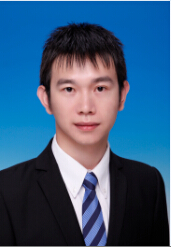
\includegraphics[width=1.8cm,height=2.6cm]{myphoto.jpg}}\\
  \zihao{5}籍贯: & \zihao{5}湖北荆门 & \zihao{5}民族: & \zihao{5}汉 & \\
  \zihao{5}出生年月: & \zihao{5}1991年2月 & \zihao{5}政治面貌: & \zihao{5}中共党员 & \\
  \zihao{5}电话号码: & \zihao{5}152-1083-0587 & \zihao{5}电子邮件: & \zihao{5}xiaoyifeibupt@bupt.edu.cn & \\
  \zihao{5}联系地址: & \multicolumn{3}{l}{\zihao{5}北京市海淀区西土城路10号北京邮电大学新科研楼606} & \\
\end{tabular}\par
\vspace{1.2ex}
\noindent \textbf{\zihao{-4} \heiti \faGraduationCap\ 教育背景}\par
\vspace{1.2ex}
\indent \textbf{\zihao{5}北京邮电大学网络与交换技术国家重点实验室~~计算机科学与技术~~(硕士研究生)}\hfill \zihao{5}2013.9-2016.3
\begin{itemize}[topsep=0.3em, leftmargin=3pc]
  \setlength{\itemsep}{0pt}
  \setlength{\parsep}{4pt}
  \setlength{\parskip}{4pt}
  \item \zihao{5}2013-2014学年度校级一等奖学金
  \item \zihao{5}2013-2014学年度优秀研究生干部
  \item \zihao{5}2014-2015学年度优秀团支书
  \item \zihao{5}担任团支部书记期间带领支部荣获优秀研究生团支部,北京市“先锋杯”优秀团支部
\end{itemize}\par
\indent \textbf{\zihao{5}北京邮电大学~~信息与计算科学~~(本科)}\hfill \zihao{5}2009.9-2013.6
\begin{itemize}[topsep=0.3em, leftmargin=3pc]
  \setlength{\itemsep}{0pt}
  \setlength{\parsep}{4pt}
  \setlength{\parskip}{4pt}
  \item \zihao{5}2011-2012学年度校级三等奖学金和2010-2011学年度校级三等奖学金
  \item \zihao{5}2011-2012校级优秀学生干部和2010-2011校级优秀学生干部
  \item \zihao{5}担任学生会科技部部长期间获“优秀部长”称号
\end{itemize}
\noindent \textbf{\zihao{-4} \heiti \faCogs\ 个人能力}
\begin{itemize}[topsep=0.3em, leftmargin=3pc]
  \setlength{\itemsep}{0pt}
  \setlength{\parsep}{4pt}
  \setlength{\parskip}{4pt}
  \item \zihao{5}熟练掌握Linux平台上的C/C++程序设计语言,对标准库和面向象编程具有一定的理解
  \item \zihao{5}熟练掌握 Java程序设计语言
  \item \zihao{5}熟悉网络编程、多线程编技术
  \item \zihao{5}了解Python/shell等脚本语言
  \item \zihao{5}通过大学英语六级,具有流利的英文听说读写译能力
\end{itemize}
\noindent \textbf{\zihao{-4} \heiti \faBriefcase\ 实习经历}\par
\vspace{1.2ex}
\uline{\zihao{5}2015.7——2015.8~~~~~~~~~~\bf{网之易信息技术(北京)有限公司}\hfill \bf{\zihao{-5}软件研发实习生}}
\begin{itemize}[topsep=0.3em, leftmargin=3pc]
  \setlength{\itemsep}{0pt}
  \setlength{\parsep}{4pt}
  \setlength{\parskip}{4pt}
  \item \zihao{5}MySQL Proxy 是一个位于Client端和Server端的中间层代理,底层使用C实现网络连接、连接池等核心操作,并暴露出部分数据结构提供给Lua,用以实现常用的功能逻辑。实习所在的项目组是是对MySql proxy进行二次开发,改进了连接池操作,并增加了故障检测、转移以及简单的读写分离功能。
  \item \zihao{5}将处理连接的模型修改为非阻塞IO,事件驱动模型,增加并发能力
  \item \zihao{5}使用Lua脚本编写测试逻辑,使用MySQL Test语法编写测试用例,完成Proxy复杂的测试
  \item \zihao{5}开发工具:Linux、C、lua、MySQL Test
\end{itemize}\par
\uline{\zihao{5}2014.7——2015.4~~~~~~~~~~\bf{三星电子中国通信研究院}\hfill \bf{\zihao{-5}软件研发实习生}}
\begin{itemize}[topsep=0.3em, leftmargin=3pc]
  \setlength{\itemsep}{0pt}
  \setlength{\parsep}{4pt}
  \setlength{\parskip}{4pt}
  \item \zihao{5}实习所在的项目组是负责将客户端传入的音频信号经过各个功能单元处理之后形成文字信息(ASR,Auto Speech Recognition),并在此基础上进行一定的自然语言理解(NLU, Natural Language Understanding)
  \item \zihao{5}设计和开发ASR+NLU系统引擎,引擎的功能包括通过管理页面或者shell脚本控制每个处理单元的启动和关闭、监听每个处理单元的工作状态、维持各个处理单元之间的数据通信以及每个处理单元与引擎的通信
  \item \zihao{5}设计和开发Android平台ASR+NLU系统管理工具
  \item \zihao{5}开发工具:Linux、C/C++、Java、JNI、jetty、Android ADT
\end{itemize}
\noindent \textbf{\zihao{-4} \heiti \faUniversity\ 实验室项目}\par
\vspace{1.2ex}
\uline{\zihao{5}2013.9——2015.7~~~~~~~~~~\bf{Defect Testing System(DTS)} \hfill \bf{\zihao{5}国家863项目}}
\begin{itemize}[topsep=0.3em, leftmargin=3pc]
  \setlength{\itemsep}{0pt}
  \setlength{\parsep}{4pt}
  \setlength{\parskip}{4pt}
  \item \zihao{5}DTS(软件缺陷测试系统)是在多个国家863项目和自然基金项目的资助下进行的,采用全新的软件测试理念、应用国际上目前主流的软件测试技术,是国内第一套基于软件缺陷的测试工具,目前可以检测故障和安全漏洞数百种缺陷模式,应用DTS可大大提高软件的测试效率和软件质量
  \item \zihao{5}主要负责DTS对C语言安全模式的支持,应用 JavaCC对预处理文件生成抽象语法树 ,扫描可能产生异常的节点
  \item \zihao{5}开发工具:Java、Eclipse
\end{itemize}\par
\uline{\zihao{5}2013.2——2013.8~~~~~~~~~~\bf{基于Android平台的WebView组件的封装} \hfill \bf{\zihao{5}科技重大专项}}
\begin{itemize}[topsep=0.3em, leftmargin=3pc]
  \setlength{\itemsep}{0pt}
  \setlength{\parsep}{4pt}
  \setlength{\parskip}{4pt}
  \item \zihao{5}WebView是Android和iOS系统中的一个组件,相当于是一个迷你Web浏览器,通过封装WebView组件,使其对上层移动应用提供更多功能,开发者基于扩展后的WebView组件可用web技术(HTML/JavaScript/CSS)快速完成移动应用开发
  \item \zihao{5}本次封装主要是基于当前互联网上比较成熟的移动中间件(PhoneGap)来进行插件扩展,完成了通话,短信,彩信以及电子邮件等基本应用的插件扩展,并且基于这些已经完成的插件整合开发了一个Web App,用于实现具有行业特色的用户业查询模块,扫描包含特定信息的二维码实现信息的查询和修改
  \item \zihao{5}开发工具:Java、Android SDK
\end{itemize}
\noindent \textbf{\zihao{-4} \heiti \faCode\ 个人项目}
\begin{itemize}[topsep=0.3em, leftmargin=3pc]
  \setlength{\itemsep}{0pt}
  \setlength{\parsep}{4pt}
  \setlength{\parskip}{4pt}
  \item \zihao{5}xhttpd©是一个简单高效的HTTP Server,在Linux平台下C++语言开发,基于非阻塞IO、事件驱动和one loop per thread模型,利用epoll的ET模式,支持GET和POST方法、多线程、公共网关接口(CGI)、文件和目录的访问、404等错误处理,项目地址:https://github.com/xiaoyifeibupt/xhttpd
  \item \zihao{5}xMultiThread©是一套Linux平台下利用C++语言封装的线程相关组件,利用RAII技术,包括线程库,互斥锁(MutexLock),条件变量(Condition),无界阻塞队列(BlockingQueue),同步计数器(CountDownLatch)等,项目地址:https://github.com/xiaoyifeibupt/xMultiThread
  \item \zihao{5}lcSpider是一个利用Python语言开发的爬虫工具,用于获取LeetCode和LintCode自己通过的题目和答案,项目地址:https://github.com/xiaoyifeibupt/LCSpider
  \item \zihao{5}个人主页http://xiaoyifeibupt.github.io/ ,其中博客部分为自己平常学习过程中做的笔记,内容涉及Linux 、C++、HTTP、设计模式等。
  \item \zihao{5}GitHub https://github.com/xiaoyifeibupt
\end{itemize}

\end{document}
